\section{Test-and-Fallback in Depth}

The test-and-fallback algorithms are the paper's adaptive robustness
mechanism, and the object of the theory in Section 7. This section gives
their first empirical study: the robustness envelope they achieve, a
counter-intuitive failure of the acceptance threshold, its
recalibration, and the resolution limit that recalibration exposes ---
the empirical face of the budget--stakes law we prove in Section 7.
Throughout, the \(\ell_1\) test is the empirical-\(\ell_1\)
proof-of-concept the original authors also fall back to (Section 2.2).

\subsection{The robustness envelope}

We sweep advice error \(\ell_1(p,q)\) on few-types instances
(\(n=2000\), \(r=8\), prefix \(k=200\), 40 trials) and compare blind
FollowPrediction, TestAndMatch (Choo and BEM variants), and the Ranking
floor (\textbf{Figure 3}). The picture is textbook. FollowPrediction
degrades \emph{linearly}, from \(1.000\) at perfect advice to \(0.453\)
at \(\ell_1\!\approx\!1.1\) --- well \emph{below} the advice-free floor
(\(\approx 0.99\)). TestAndMatch instead stays on the \textbf{upper
envelope}: it captures the benefit when advice is good and, when advice
is bad, its prefix test rejects it and it falls back to Ranking, never
crashing (BEM \(0.998\to0.969\); Choo \(1.000\to0.991\) across the same
sweep). This is the adaptive counterpart of the structural robustness of
Section 3: the engineered mechanism that MPD lacked.

\begin{figure}
\centering
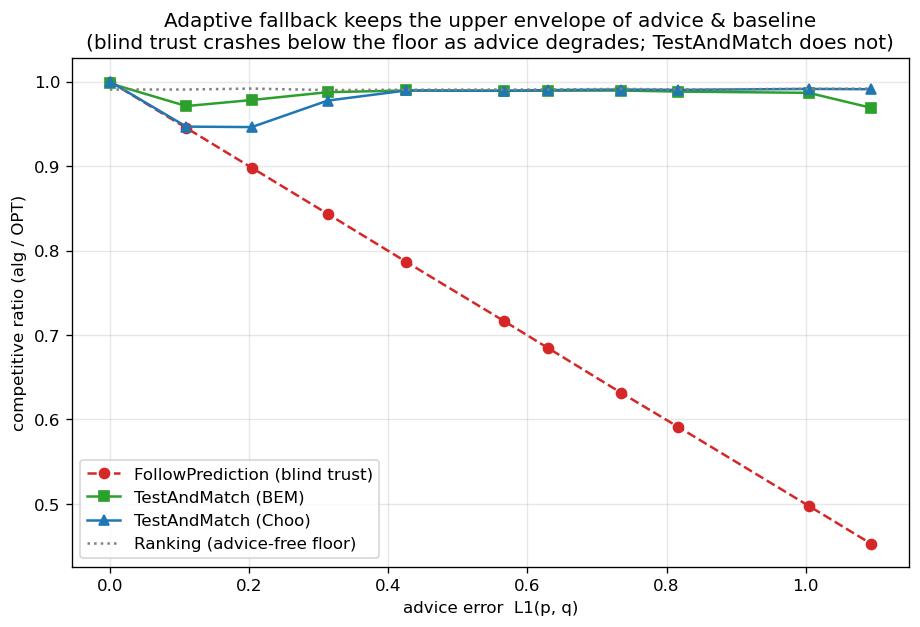
\includegraphics[width=0.7\linewidth,height=\textheight,keepaspectratio,alt={The robustness envelope: blind FollowPrediction crashes below the advice-free floor as advice error grows; TestAndMatch stays on the upper envelope.}]{../../../results/choo_bem_envelope.png}
\caption{The robustness envelope: blind FollowPrediction crashes below
the advice-free floor as advice error grows; TestAndMatch stays on the
upper envelope.}
\end{figure}

\subsection{A threshold that is too lenient on average-case
inputs}

What does the ``test then maybe fall back'' machinery cost, and does a
better test make a better decision? We sweep the prefix (testing) size
\(k\) at \emph{borderline} advice (\(\eta=0.15\), true
\(\ell_1\!\approx\!0.16\)) --- the regime where the test must work
hardest (\textbf{Figure 4}). Counter-intuitively, \textbf{a larger, more
accurate test makes the \emph{worse} decision}: as \(k\) grows
\(25\to100\to200\to800\), the ratio \emph{falls} \(0.992\to0.981\to
0.969\to0.956\) and the misjudgement rate (against an empirical oracle:
should we have followed, given that following actually underperformed
the baseline here?) \emph{rises} \(0.00\to0.13\to0.33\to0.60\).

\begin{figure}
\centering
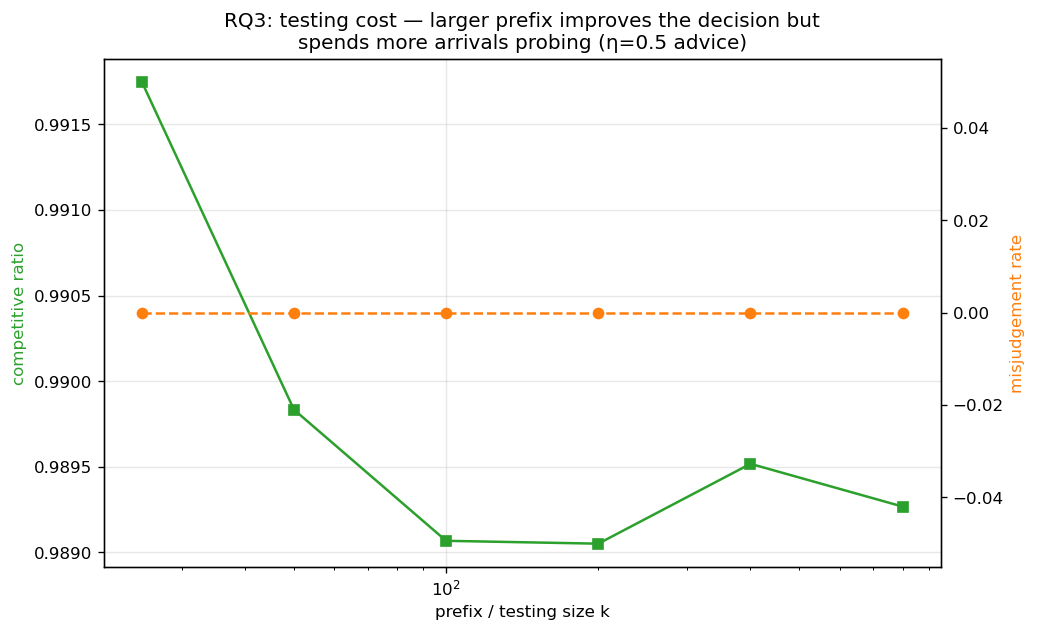
\includegraphics[width=0.7\linewidth,height=\textheight,keepaspectratio,alt={Testing cost at borderline advice: under the worst-case-calibrated threshold, a larger and more accurate prefix test makes the worse decision.}]{../../../results/choo_bem_prefix.png}
\caption{Testing cost at borderline advice: under the
worst-case-calibrated threshold, a larger and more accurate prefix test
makes the \emph{worse} decision.}
\end{figure}

The mechanism is a real and reportable finding. The Choo/BEM acceptance
threshold \(\tau\) is calibrated to the \emph{worst-case} baseline
\(\beta\approx0.696\). But on these average-case instances the baseline
is \(\approx0.99\) (Section 3, F3), so the \emph{empirical} break-even
--- the advice error at which following stops beating the baseline ---
sits at \(\ell_1\approx0\), far below \(\tau\). A small, noisy prefix
over-estimates \(\ell_1\) and \emph{accidentally rejects} the borderline
advice, landing on the strong Ranking floor; a large, accurate prefix
correctly measures \(\ell_1\approx0.16<\tau\) and so \textbf{accepts}
the mildly-bad advice the worst-case threshold deems acceptable --- and
underperforms the baseline. On strong-baseline inputs the
worst-case-calibrated threshold is too \emph{lenient}, and improving the
test's accuracy only makes the algorithm follow that miscalibrated
threshold more faithfully.

\subsection{Recalibration, and the resolution limit it
exposes}

The natural fix is to recalibrate \(\tau\) to the \emph{measured}
baseline \(\hat\beta\) (the mean empirical Ranking ratio on a small
calibration sample) rather than the worst-case \(\beta\). On the same
instances this eliminates the pathology: at borderline advice the
worst-case threshold's misjudgement climbs \(0.03\to1.00\) as the prefix
grows and its ratio drops to \(0.920\), whereas the recalibrated
threshold holds misjudgement \(=0.00\) at every prefix size and ratio
\(\approx0.986\) --- a larger prefix no longer hurts.

But recalibration exposes a deeper, honest limit. At \emph{perfect}
advice (\(\ell_1=0\)) the worst-case threshold scores \(1.000\) (it
accepts and follows), while the recalibrated one scores only \(0.987\):
the recalibrated threshold \(\tau\approx 2(1-\hat\beta)\approx 0.028\)
is \emph{smaller than the empirical-\(\ell_1\) estimator's own noise
floor} (\(\approx 0.05\)--\(0.13\) at this prefix and support), so the
test can never confidently \emph{accept} --- it rejects everything,
including perfect advice, and effectively always plays the baseline. In
other words:

\begin{quote}
On strong-baseline instances, no practical empirical-\(\ell_1\)
threshold can both capture the consistency upside and stay safe: the
upside is tiny (the baseline is already \(\approx\mathrm{OPT}\)) and
sits \emph{below the estimator's resolution}. The worst-case threshold
over-accepts (§5.2); the recalibrated threshold over-rejects; and a
better tester only follows whichever threshold more faithfully.
\end{quote}

Section 7 turns this phenomenon into a two-sided law. The resolution
limit above is specific to the empirical-\(\ell_1\) statistic --- §7.7
shows that class is blind for a structural reason (the plug-in distance
saturates at \(k \ll r\) regardless of advice quality) --- but the
deeper point holds for \emph{any} test on a sublinear prefix: the
follow/fallback decision costs a prefix of
\(\tilde\Theta(\theta/\delta^2)\), and on strong-baseline instances like
these the stakes \(\delta\) are so small that the price exceeds the
horizon. Section 5 is the empirical shadow; Section 7 is the law.

\subsection{The dynamic combiner is dominated, and shows why matching
needs
test-then-commit}

Finally we benchmark the Chłędowski-style dynamic combiner (Section 2.2)
to contextualize the \emph{commit-once} structure of test-and-fallback.
In its intended robust tuning the combiner sits exactly on the floor
(\(0.990\) across all advice quality on few-types): it never crashes,
but captures \emph{none} of the consistency upside --- strictly
dominated by TestAndMatch on the good-advice side and equal to it on the
bad side.

More instructively, an \emph{eager} combiner that switches experts
mid-stream reveals a penalty specific to irrevocable problems. With
perfect advice, eager switching scores \(0.927\) --- \emph{below both}
the pure follower (\(1.000\)) and the pure baseline (\(0.958\); verified
in \texttt{tests/test\_combiner\_small.py}) --- because switching from
Ranking to Mimic mid-run lands the committed matching in an
\emph{incompatible hybrid}: the Mimic plan's slots are already
half-consumed by the Ranking phase, and the Ranking progress is
abandoned. In an irrevocable problem the follow/fallback decision must
be made \emph{before} the bulk of the commitments, not adapted across
them --- which is precisely why Choo/BEM test on a prefix and then
\emph{commit}, rather than switching dynamically as the caching-style
combiner does. The dynamic combiner that is cheap worst-case insurance
for caching does not port cleanly to matching, and the unified benchmark
shows why.
